\section{Black Box Expression Compiler}

\subsection{Overview}

The Black Box Expression Compiler is a multi-stage compilation pipeline that transforms FASTEXPR source code into validated, optimized expressions with operators and data fields. The compiler operates as a black box, taking source code as input and producing a final expression through a series of well-defined stages.

\subsection{Compiler Architecture}

The compiler follows a traditional multi-stage architecture:

\begin{enumerate}
    \item \textbf{Lexical Analysis}: Tokenizes source code
    \item \textbf{Parsing}: Builds Abstract Syntax Tree (AST)
    \item \textbf{Semantic Analysis}: Validates types and operator-field compatibility
    \item \textbf{Intermediate Representation (IR)}: Transforms AST to IR
    \item \textbf{Code Generation}: Generates final expression
    \item \textbf{Optimization}: Applies optimizations (optional)
\end{enumerate}

\subsection{Compiler Pipeline}

\subsubsection{Stage 1: Lexical Analysis}

The lexical analyzer tokenizes the input source code into a sequence of tokens.

\textbf{Token Types:}
\begin{itemize}
    \item \texttt{OPERATOR}: Function names (e.g., \texttt{ts\_rank}, \texttt{rank})
    \item \texttt{FIELD}: Data field identifiers (e.g., \texttt{anl49\_1stfiscalquarterearningspershare})
    \item \texttt{LITERAL}: Numeric constants (e.g., \texttt{20}, \texttt{3.14})
    \item \texttt{ARITHMETIC}: Arithmetic operators (\texttt{+}, \texttt{-}, \texttt{*}, \texttt{/}, \texttt{>=}, \texttt{<=}, etc.)
    \item \texttt{PAREN}: Parentheses (\texttt{(}, \texttt{)})
\end{itemize}

\textbf{Token Structure:}
\begin{equation}
\text{Token} = (\text{type}, \text{value}, \text{position})
\end{equation}

where:
\begin{itemize}
    \item \textit{type}: Token type identifier
    \item \textit{value}: Token string value
    \item \textit{position}: Character position range $(start, end)$
\end{itemize}

\subsubsection{Stage 2: Parsing}

The parser builds an Abstract Syntax Tree (AST) from tokens using recursive descent parsing.

\textbf{AST Node Types:}
\begin{itemize}
    \item \texttt{function}: Operator calls with arguments
    \item \texttt{field}: Data field references
    \item \texttt{literal}: Constant values
    \item \texttt{arithmetic}: Arithmetic operations
\end{itemize}

\textbf{Parsing Algorithm:}
\begin{enumerate}
    \item Handle parentheses and precedence
    \item Identify arithmetic operators (lowest precedence first)
    \item Parse function calls: \texttt{operator(args)}
    \item Parse field references and literals
    \item Build tree structure recursively
\end{enumerate}

\textbf{Operator Precedence:}
\begin{equation}
\begin{aligned}
\text{Precedence}(\texttt{\^}) &= 4 \\
\text{Precedence}(\texttt{*}, \texttt{/}, \texttt{\%}) &= 3 \\
\text{Precedence}(\texttt{+}, \texttt{-}) &= 2 \\
\text{Precedence}(\texttt{>}, \texttt{<}, \texttt{>=}, \texttt{<=}, \texttt{==}, \texttt{!=}) &= 1 \\
\text{Precedence}(\texttt{\&\&}, \texttt{||}) &= 0
\end{aligned}
\end{equation}

\subsubsection{Stage 3: Semantic Analysis}

Semantic analysis validates the AST for correctness:

\textbf{Validation Checks:}
\begin{enumerate}
    \item \textbf{Operator Existence}: Verify operators exist in operator dictionary
    \item \textbf{Field Existence}: Verify data fields exist in field dictionary
    \item \textbf{Type Compatibility}: Check operator scope matches field type
    \begin{itemize}
        \item \texttt{REGULAR} fields work with regular operators
        \item \texttt{MATRIX} fields work with time-series operators (\texttt{ts\_*})
        \item \texttt{VECTOR} fields work with vector operators (\texttt{vec\_*})
    \end{itemize}
    \item \textbf{Arity Checking}: Verify correct number of arguments
    \item \textbf{Parentheses Balance}: Ensure balanced parentheses
\end{enumerate}

\textbf{Type Compatibility Matrix:}

\begin{table}[h]
\centering
\begin{tabular}{l|c|c|c}
\textbf{Operator Scope} & \textbf{REGULAR} & \textbf{MATRIX} & \textbf{VECTOR} \\
\hline
\texttt{REGULAR} & \checkmark & \checkmark & \checkmark \\
\texttt{MATRIX} & \checkmark & \checkmark & \times \\
\texttt{VECTOR} & \times & \times & \checkmark \\
\end{tabular}
\caption{Operator-Field Type Compatibility}
\end{table}

\subsubsection{Stage 4: Intermediate Representation (IR)}

The IR stage transforms the AST into an intermediate representation that separates structure from syntax.

\textbf{IR Node Types:}
\begin{itemize}
    \item \texttt{operator\_call}: Operator invocations with typed arguments
    \item \texttt{field\_ref}: Field references with metadata
    \item \texttt{literal}: Constant values
    \item \texttt{arithmetic}: Arithmetic operations with typed operands
\end{itemize}

\textbf{IR Structure:}
\begin{equation}
\text{IRNode} = \begin{cases}
\text{operator\_call}(op, [args], metadata) \\
\text{field\_ref}(field\_id, metadata) \\
\text{literal}(value) \\
\text{arithmetic}(op, left, right)
\end{cases}
\end{equation}

\textbf{Metadata includes:}
\begin{itemize}
    \item Field types (\texttt{REGULAR}, \texttt{MATRIX}, \texttt{VECTOR})
    \item Operator scope information
    \item Validation results
    \item Type inference results
\end{itemize}

\subsubsection{Stage 5: Code Generation}

Code generation produces the final FASTEXPR expression from the IR.

\textbf{Generation Algorithm:}
\begin{algorithmic}
\Function{GenerateExpression}{IRNode}
    \If{IRNode.type = operator\_call}
        \State $args \gets \text{map}(\text{GenerateExpression}, \text{IRNode.arguments})$
        \State \Return $\text{IRNode.operator}(args)$
    \ElsIf{IRNode.type = field\_ref}
        \State \Return $\text{IRNode.field\_id}$
    \ElsIf{IRNode.type = literal}
        \State \Return $\text{str}(\text{IRNode.value})$
    \ElsIf{IRNode.type = arithmetic}
        \State $left \gets \text{GenerateExpression}(\text{IRNode.left})$
        \State $right \gets \text{GenerateExpression}(\text{IRNode.right})$
        \State \Return $(left \text{ IRNode.op } right)$
    \EndIf
\EndFunction
\end{algorithmic}

\subsubsection{Stage 6: Optimization}

Optional optimization stage applies transformations to improve expression efficiency.

\textbf{Optimization Techniques:}
\begin{enumerate}
    \item \textbf{Redundant Parentheses Removal}: Simplify nested parentheses
    \item \textbf{Constant Folding}: Evaluate constant expressions at compile time
    \item \textbf{Operator Fusion}: Combine compatible operators
    \item \textbf{Dead Code Elimination}: Remove unreachable code
\end{enumerate}

\textbf{Optimization Example:}
\begin{align}
\text{Before:} \quad & \texttt{((ts\_rank(field, 20)))}\\
\text{After:} \quad & \texttt{ts\_rank(field, 20)}
\end{align}

\subsection{Compilation Result}

The compiler returns a \texttt{CompilationResult} containing:

\begin{itemize}
    \item \textbf{success}: Boolean indicating compilation success
    \item \textbf{source\_code}: Original source code
    \item \textbf{tokens}: Tokenized representation
    \item \textbf{ast}: Abstract Syntax Tree
    \item \textbf{ir}: Intermediate Representation
    \item \textbf{final\_expression}: Generated FASTEXPR expression
    \item \textbf{errors}: List of compilation errors
    \item \textbf{warnings}: List of compilation warnings
    \item \textbf{stage\_reached}: Last successful compilation stage
    \item \textbf{metadata}: Additional information (operator count, field count, complexity)
\end{itemize}

\subsection{Compilation Flow Diagram}

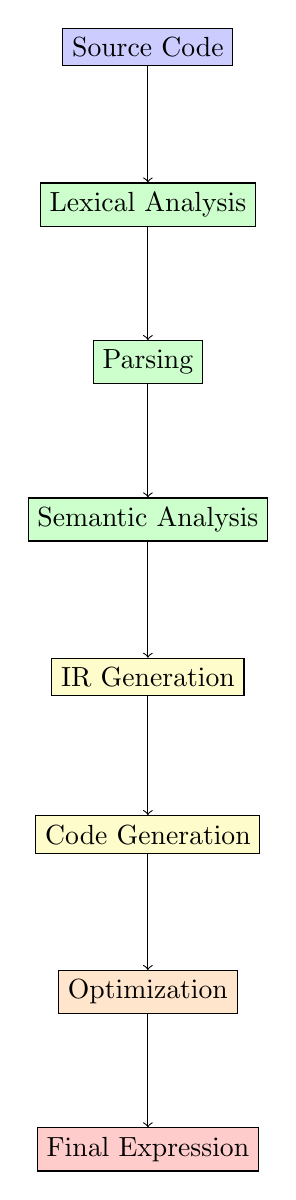
\begin{tikzpicture}[node distance=2cm, auto]
    \node [rectangle, draw, fill=blue!20] (source) {Source Code};
    \node [rectangle, draw, fill=green!20, below of=source] (lex) {Lexical Analysis};
    \node [rectangle, draw, fill=green!20, below of=lex] (parse) {Parsing};
    \node [rectangle, draw, fill=green!20, below of=parse] (semantic) {Semantic Analysis};
    \node [rectangle, draw, fill=yellow!20, below of=semantic] (ir) {IR Generation};
    \node [rectangle, draw, fill=yellow!20, below of=ir] (codegen) {Code Generation};
    \node [rectangle, draw, fill=orange!20, below of=codegen] (optimize) {Optimization};
    \node [rectangle, draw, fill=red!20, below of=optimize] (result) {Final Expression};
    
    \draw [->] (source) -- (lex);
    \draw [->] (lex) -- (parse);
    \draw [->] (parse) -- (semantic);
    \draw [->] (semantic) -- (ir);
    \draw [->] (ir) -- (codegen);
    \draw [->] (codegen) -- (optimize);
    \draw [->] (optimize) -- (result);
\end{tikzpicture}

\subsection{Error Handling}

The compiler provides detailed error reporting at each stage:

\textbf{Error Types:}
\begin{itemize}
    \item \texttt{invalid\_operator}: Unknown operator name
    \item \texttt{invalid\_field}: Unknown data field
    \item \texttt{type\_mismatch}: Operator-field type incompatibility
    \item \texttt{unbalanced\_parens}: Mismatched parentheses
    \item \texttt{invalid\_syntax}: General syntax errors
    \item \texttt{compilation\_error}: Runtime compilation errors
\end{itemize}

\textbf{Error Structure:}
\begin{equation}
\text{Error} = (\text{type}, \text{message}, \text{position}, \text{suggested\_fix})
\end{equation}

\subsection{Complexity Metrics}

The compiler calculates expression complexity:

\textbf{Complexity Formula:}
\begin{equation}
\text{Complexity} = \max(\text{depth}(node)) + \sum \text{operators}(node)
\end{equation}

where:
\begin{itemize}
    \item $\text{depth}(node)$: Maximum depth of AST
    \item $\text{operators}(node)$: Total number of operators
\end{itemize}

\subsection{Usage Example}

\begin{lstlisting}[language=Python, caption=Compiler Usage]
from generation_two.core.expression_compiler import ExpressionCompiler
from generation_two.core.fast_expr_ast import FASTEXPRParser

# Initialize parser with operators and fields
parser = FASTEXPRParser(operators=operators, data_fields=fields)

# Create compiler
compiler = ExpressionCompiler(parser)

# Compile expression
source = "ts_rank(field_id, 20)"
result = compiler.compile(source, optimize=True)

if result.success:
    print(f"Final expression: {result.final_expression}")
    print(f"Complexity: {result.metadata['complexity']}")
else:
    for error in result.errors:
        print(f"Error: {error.message}")
\end{lstlisting}

\subsection{Integration with Template Generation}

The compiler integrates with the template generation system:

\begin{enumerate}
    \item \textbf{Template Validation}: Compile templates to validate syntax
    \item \textbf{Expression Transformation}: Transform templates using IR
    \item \textbf{Optimization}: Optimize generated expressions
    \item \textbf{Error Feedback}: Provide detailed errors for self-correction
\end{enumerate}

\subsection{Performance Characteristics}

\textbf{Time Complexity:}
\begin{itemize}
    \item Lexical Analysis: $O(n)$ where $n$ is source length
    \item Parsing: $O(n)$ for recursive descent
    \item Semantic Analysis: $O(m)$ where $m$ is AST node count
    \item IR Generation: $O(m)$
    \item Code Generation: $O(m)$
    \item Optimization: $O(m)$ (depends on optimization level)
\end{itemize}

\textbf{Space Complexity:}
\begin{itemize}
    \item Token storage: $O(n)$
    \item AST storage: $O(m)$
    \item IR storage: $O(m)$
    \item Total: $O(n + m)$
\end{itemize}

\subsection{Future Enhancements}

\begin{itemize}
    \item Advanced optimizations (constant propagation, dead code elimination)
    \item Expression rewriting rules
    \item Type inference and checking
    \item Parallel compilation for batch processing
    \item Caching of compilation results
\end{itemize}
